\chapter{Production Node Control} \label{chapProdControl}

This chapter focuses on the problems involving the control of a production node. The control activity, from a logistic point of view, is necessary to ensure the production processes are smooth and efficient. 

\section{Performance assessment (P8)}
\textit{“If you can’t measure it, you can’t manage it”}. This famous quote of the philosopher and economist Peter Drucker clearly defines the importance of performance assessment. The aim is the modelling of processes and the measurement of their efficiency from different points of view. Here qualitative and quantitative methods are introduced to measure and understand the processes.

\subsection{Model-driven methods (D4)}

Business process modelling is a qualitative mapping activity aiming at the definition of the relationships between physical and information entities involved in any process. The modelling of production processes allows defining their interactions with operators, resources, parts and information systems. The Business Process Model and Notation (see section \ref{secBPMN} is a graphical model for this purpose using predefined symbols to model tasks, activities and interactions. Mapping a production environment:

\begin{itemize}
    \item the activities are any production or auxiliary task necessary for the realisation of the product (manufacturing, traceability, supplier and customers interactions).
    \item the events identify the step of the processes concluding an activity, and the part increases its value (e.g. the end of the production or the inbound process).
    \item the gateways describe different production path (e.g. variants of the products)
    \item the pools identify the department or the office in charge of specific tasks.

\end{itemize}

BPMN defines a qualitative map of the production processes useful for manager and practitioners to identify the way their processes are realised. The hard assessment takes place with the definition of quantitative KPIs. The KPIs used in these chapters refers to the metrics defined in \ref{secOntology}. KPIs are organised according to four classes, relevant to the logistics and operation design ~\cite{Tufano2018}:

\begin{enumerate}
    \item Logistic KPIs, evaluate the logistic impact of a certain solution. They use metrics like time, distance and the performance parameters introduced in section \ref{secOntology}.
	\item Cost KPIs, evaluate the economic sustainability of a given solution. They are expressed in \euro{} or other currency.
	\item Energy KPIs, evaluate the energy needed to feed a given solution. They use metrics as kW and kW/h.
	\item Environmental KPIs, evaluate the environmental impact of a given solution. They are expressing the equivalent $CO_2$ produced per year.

\end{enumerate}

Table \ref{tab_prod_KPIs} identifies which KPI is relevant to each problem. In general, each problem can be assessed from multiple perspectives.

% INSERT tab_prod_KPIs
\begin{figure}[hbt!]
\centering
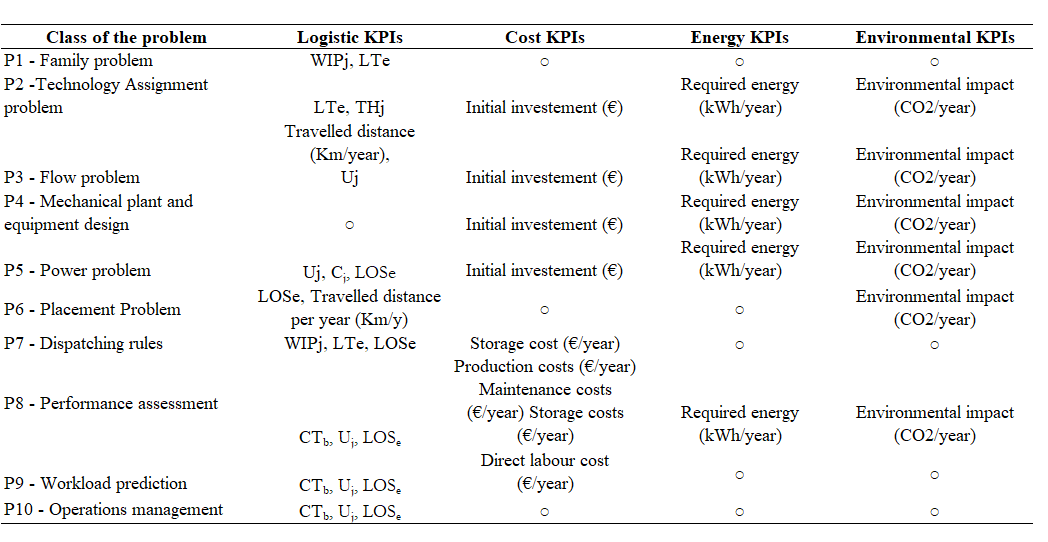
\includegraphics[width=0.9\textwidth]{sectionProduction/control_figures/tab_prod_KPIs.png}
\captionsetup{type=table}
\caption{KPIs to evaluate the solution of the problems in a production node.}
\label{tab_prod_KPIs}
\end{figure}

\subsection{Data-driven methods (D1, D2, D3, D4)}
The definition of the KPIs is a modelling activity where the definition of a BPMN may help to identify which are the KPIs essential to monitor. With the advent of Big Data, the amount of collected record can be ample, and the pure definition of the KPI neglects a significant amount of information.\par

Data-driven methods use descriptive analytics to manipulate these data and extract information. Clustering methods (see section \ref{secClustering}) allows defining clusters. In particular, having a time series of a KPIs it is possible to identify if a value diverges to out-of-control of anomalous values. These values are often associated with bottlenecks and inefficiencies of the production process. Inferential statistics (see section \ref{secStatistics}) is used to describe the behaviour of a KPI as a random variable. Almost always the value of a KPI changes, and it is relevant to identify its statistics to evaluate the robustness and steadiness of a production process. Bayesian statistic (see section \ref{secBayesianMethods}) can be used to define the statistics of a KPI when only partially reliable measurements are available. Finally, simulation approaches (e.g. Monte Carlo see section \ref{secMontecarlo}) uses different input measurement to identify the behaviour of the output from a statistical point of view.  

\section{Workload prediction (P9)}
Workload prediction aims at forecasting the value of the workload in the future. Companies rely on a demand forecast that is the starting point to derive all the other predictions. 

\subsection{Model-driven methods (D1)} \label{secDemandPatterns}
Demand forecast depends on the type of demand pattern of a part. Identifying the right demand pattern can be seen as a clustering problem (i.e. solved using data-driven methods) \cite{Mikalsen}. Figure \ref{fig_prod_demand_pattern} identifies the four demand patterns.

% INSERT fig_prod_demand_pattern
\begin{figure}[hbt!]
\centering
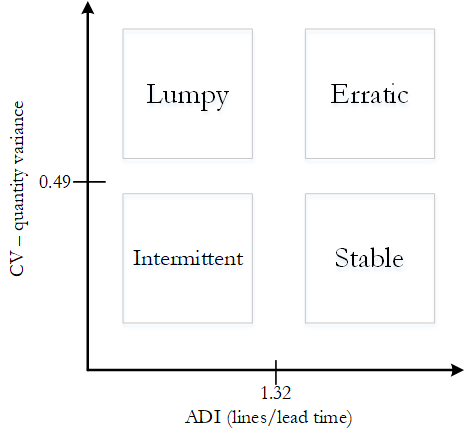
\includegraphics[width=0.7\textwidth]{sectionProduction/control_figures/fig_prod_demand_pattern.png}
\captionsetup{type=figure}
\caption{Demand patterns classification.}
\label{fig_prod_demand_pattern}
\end{figure}

Parts demand is classified by considering the variability of the quantity and the lead time between orders. These two metrics are identified by:
\begin{itemize}
    \item $ADI=\sum_{i}^{n}\frac{\gamma_i}{n}\ $;
    \item $CV^2=\left(\frac{\sigma_q}{\bar{q}}\right)^2$.
\end{itemize}

Where $\gamma_i$ is the interarrival time between two batches of goods; $\sigma_q$ is the standard deviation of the quantity for each batch, $\bar{q}$ is the average quantity for each batch. Thresholds on these metrics are identified to classify the demand ~\cite{Syntetos2005}:

\begin{itemize}
    \item Stable; these parts have a high demand frequency ($ADI\geq1.32$), and low variability in quantities ($CV^2<0.49$). Their behaviour is stable and easy to forecast.
	\item Intermittent; these parts have a low demand frequency ($ADI<1.32$), and low variability in quantities ($CV^2<0.49$). Their demand is extremely sporadic, and few data points are available making harder to predict their behaviour in the future.
	\item Erratic; these parts have a high demand frequency ($ADI\geq1.32$), and high variability in quantities ($CV^2\geq0.49$). Their demand is frequent but extremely variant in quantities. Forecasts are possible but their accuracy remains a crucial issue.
	\item Lumpy; these parts have a low demand frequency ($ADI<1.32$), and high variability in quantities ($CV^2\geq0.49$). Their behaviour is difficult to predict since there are few data points with great variability. 
\end{itemize}

Depending on the nature of the pattern demand, different analytics should be used to address the demand prediction. 

\subsection{Data-driven methods (PD1, PD2)}
Once the demand pattern has been identified, an appropriate predictive method should be chosen to make forecasts.\par

When dealing with stable and erratic parts, many data points should be available since these parts have a short average interarrival time (i.e. at least 20 data points per year). In this case, time series analysis is an appropriate methodology to analyse and forecast the demand series. In particular time series decomposition (see \ref{secTimeSeriesDecomposition}) is simple and appropriate. ARIMA models (see \ref{secARIMA}) work as well with some additional efforts in the data manipulation step since these models require stationary time series.\par

When dealing with intermittent and lumpy parts, the variance of the interarrival times is high, and it is hard to identify a robust sampling interval to estimate the demand (e.g. parts per week, per months, per year). In these cases, the probability distribution of the number of pieces per time unit cannot be approximated to the uniform, and a different distribution must be used to approximate the rareness of the events. For this reason, the Poisson distribution (see section \ref{secPoisson}) is used since it can well describe the behaviour of rare events.\par

The Poisson method identifies the probability of absorption of $x$ parts within a time interval $\tau$ having an average demand d calculated in a time interval of the same span of $\tau$. The Poisson distribution assumes $\lambda=d\tau$.

\begin{equation}
    P_{d,\tau}\left(x\right)=\frac{\lambda^xe^{-\lambda}}{x!}
\end{equation}

Alternatively, when a complex dataset $X$ containing other attributes in addition to the time series, to train a learning model (see \ref{chapLinearRegression}) can lead to more accurate results.

\section{Job scheduling (P10)} \label{secJobScheduling}
When a production plant is ready to produce, a final word is needed to assign tasks to resources. Job scheduling aims at allocating the space and time of a resource to perform a task ~\cite{Lim2014}. The nature of this problem requires a prescriptive solution which, usually, aims at minimising some objective function.

\subsection{Model-driven methods (PS1)}
Let $c_i$ be the time instant where a part $i$ is completed and $d_i$ its completion due date, the production engineer aims at minimising the lateness $L_i=c_i-d_i$.\par

Many optimisation algorithms perform this assignment by setting the value of the decision problem $P$:

\begin{equation}
   \begin{split}
   x_s=\left\{
                \begin{array}{ll}
                  1\ & if\ job\ j\ assigned\ to\ resource\ i\\
                  0 & otherwise\\
                \end{array}
              \right.
   \end{split}
\end{equation}

\begin{equation}
    \min{z}
\end{equation}

\begin{equation}
    \sum_{i=1}^{n}{p_{ij}x_{ij}\le z,\ i=1,\ldots,m}
\end{equation}

\begin{equation}
    \sum_{i=1}^{m}{x_{ij}=1,\ j=1,\ldots,n}
\end{equation}

\begin{equation}
    x_{ij}\in\left\{0,1\right\}i=1,\ldots,m\ ;j=1,\ldots,n
\end{equation}

The problem $P$ usually embeds many other constraints to describe industry-oriented specifics which prevents from the feasibility of a solution (e.g. setup time, machines dedicated to specific tasks, scheduling priorities). Job scheduling is almost entirely prescriptive, and many contributions illustrate models, optimal and suboptimal algorithms to get feasible solutions ~\cite{Pinedo2009}.

\section{Applications} 
This section illustrates the application of the methodologies above to design the control systems in two different production nodes. The first production node works in the catering sector, while the second operates in the 3PL of the automotive industry.

\subsection{Control of a food catering plant} \label{secFoodCateringControl}

\subsubsection{Performance assessment}

The collection of historical data and time series from the company’s ERP is a crucial activity to control system a catering plant. Unfortunately, the ERP of the company may not include the definition of the production cycles of the items. For this reason, a monitoring campaign helps to collect information to model the processes and to populate a relational database structured as in section \ref{secRelationalModelProduction}. Figure \ref{fig_prod_CAMST_ER} illustrates the ER structure obtained after monitoring the production processes. The database maps 213 customers, 29 delivery routes, 500 products, and more than 800 production orders on a time horizon of a week.

% INSERT fig_prod_CAMST_ER
\begin{figure}[hbt!]
\centering
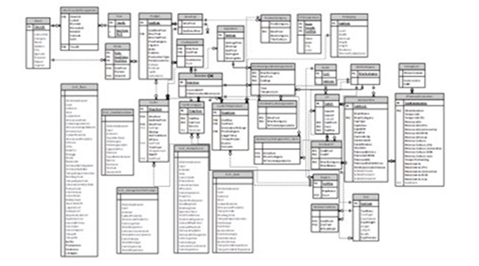
\includegraphics[width=0.7\textwidth]{sectionProduction/control_figures/fig_prod_CAMST_ER.png}
\captionsetup{type=figure}
\caption{ER model of a production node.}
\label{fig_prod_CAMST_ER}
\end{figure}

The production processes have been, also, modelled from a qualitative point of view by using a business process model. Logistics and operations processes are highly related to the temperature profile of the products (cook-warm, cook-chill, cook-chill-re-warm). Figure \ref{fig_prod_CAMST_flowchart} shows that depending on the temperature profile, products must follow different physical paths.

% INSERT fig_prod_CAMST_flowchart
\begin{figure}[hbt!]
\centering
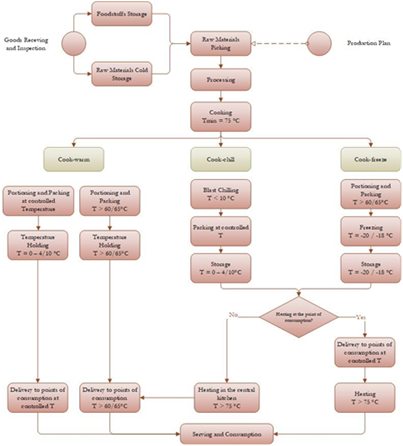
\includegraphics[width=0.7\textwidth]{sectionProduction/control_figures/fig_prod_CAMST_flowchart.png}
\captionsetup{type=figure}
\caption{Demand patterns classification.}
\label{fig_prod_CAMST_flowchart}
\end{figure}

After modelling the processes, the production flows and tasks appeared more evident to the management and the analysts. It was, then, possible to perform a quantitative analysis by defining KPIs on the single product or process ~\cite{Tufano2018}. Figure \ref{fig_prod_CAMST_performance1} illustrates a visual KPIs representing the average processing time (on the x-axis) and the average cost (on the y-axes) for each product. They both are random variable represented as error bars of the dot-plot. Besides, the dashboard shows both the Pareto curve of average times and costs, highlighting that a small number of parts generates the most considerable workload in terms of time and costs.

% INSERT fig_prod_CAMST_performance1
\begin{figure}[hbt!]
\centering
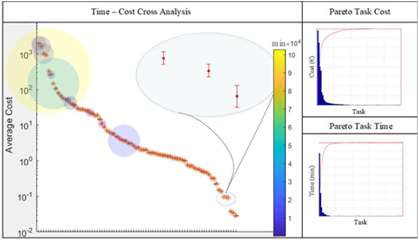
\includegraphics[width=0.7\textwidth]{sectionProduction/control_figures/fig_prod_CAMST_performance1.png}
\captionsetup{type=figure}
\caption{Dashboard of KPIs for time and costs of a catering plant.}
\label{fig_prod_CAMST_performance1}
\end{figure}

Another visual analytic tool (see Figure \ref{fig_prod_CAMST_performance2}) allows identifying the energy and environmental performance for each resource of the food plant. The histogram identifies the consumption of electric energy and gas, together with the estimate of the environmental impact measured in equivalent $CO_2$ for each production task identified by the monitoring campaign. This way, it is possible to determine which tasks and which resources need to be carefully managed to limit energy consumption.

% INSERT fig_prod_CAMST_performance2
\begin{figure}[hbt!]
\centering
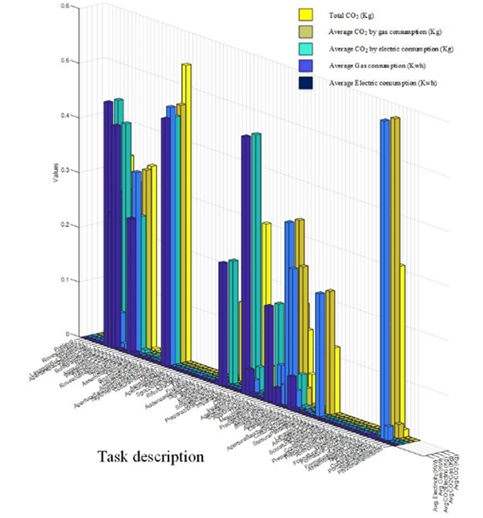
\includegraphics[width=0.7\textwidth]{sectionProduction/control_figures/fig_prod_CAMST_performance2.png}
\captionsetup{type=figure}
\caption{Energy and environmental impact for each production task.}
\label{fig_prod_CAMST_performance2}
\end{figure}

\subsubsection{Workload prediction}
Once a set of KPIs to assess the performance of the system has been identified, it is necessary to classify and make forecasts on the demand that guide any other control or design step. Historical data are collected and organised to define the value of $ADI$ and $CV^2$ for each part. The dot-plot in Figure \ref{fig_prod_CAMST_demandPatterns} identifies each product with a dot where the x- and y-axes represent the $ADI$, and $CV^2$ calculated within the reference time horizon of the dataset (one week). The size of the dot represents the number of lines (i.e. the number of orders) for each part; the bigger the dot, the higher the number of orders. The heatmap on the right pf Figure \ref{fig_prod_CAMST_demandPatterns} identifies the demand pattern of the entire production system. In this case, the demand is mainly intermittent, with low variability but significant time spans between orders of the same part. The production system has, then, to be flexible, allowing the production of the same average quantity of a vast product mix.\footnote{The source code of Figure \ref{fig_prod_CAMST_demandPatterns} is available \href{https://github.com/aletuf93/logproj/blob/master/examples/PROD_02\%20Demand\%20patterns.ipynb}{here}.}

% INSERT fig_prod_CAMST_demandPatterns
\begin{figure}[hbt!]
\centering
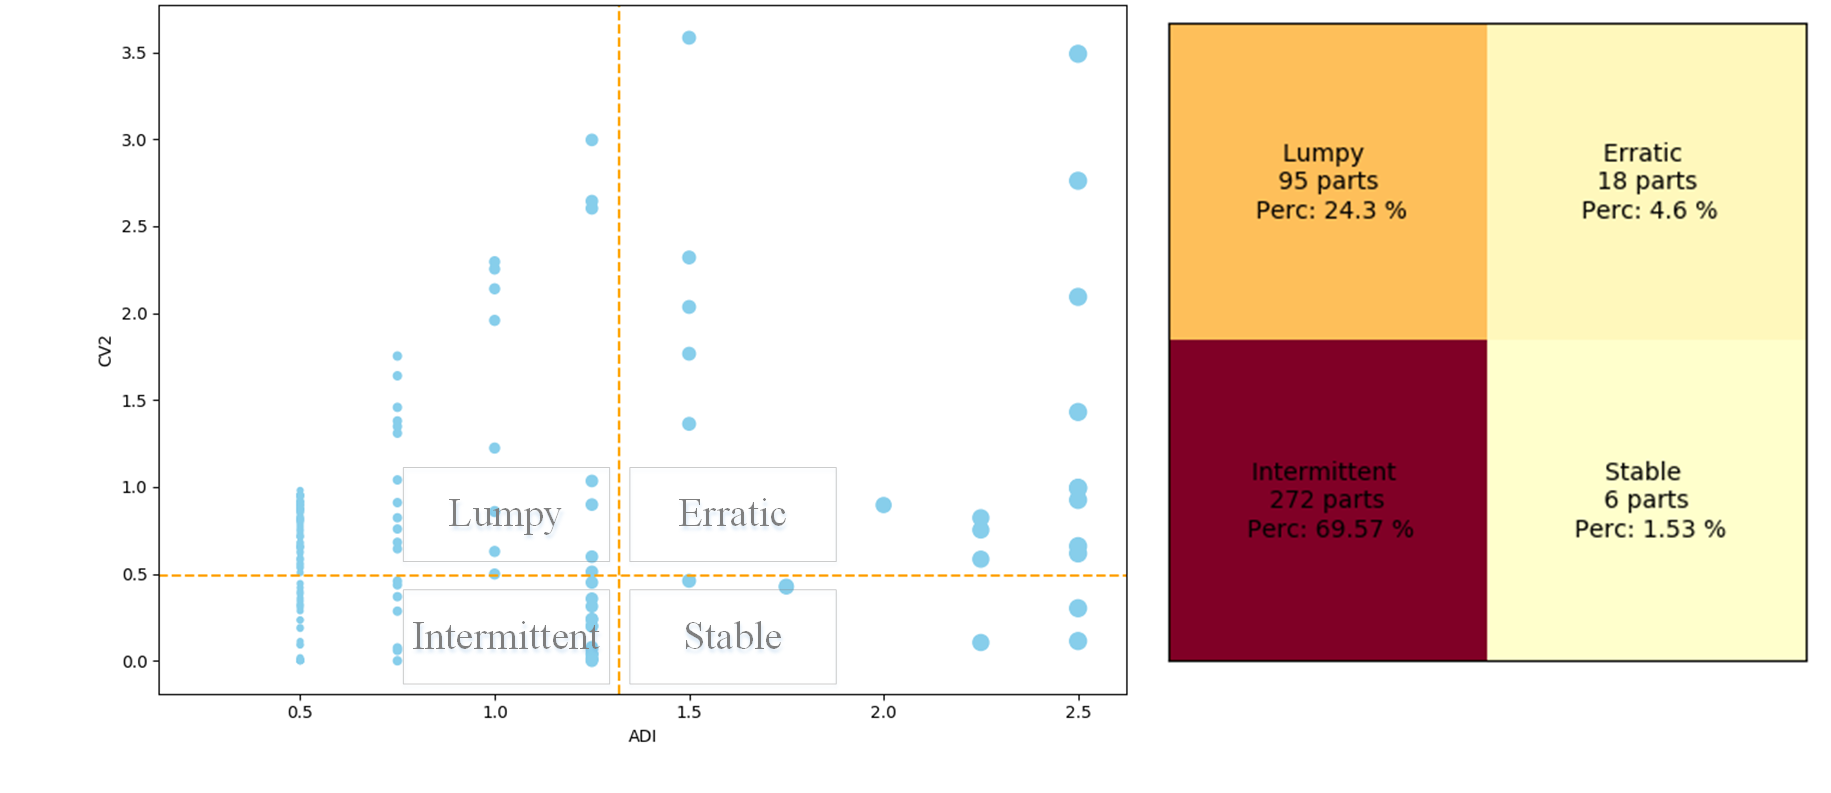
\includegraphics[width=0.9\textwidth]{sectionProduction/control_figures/fig_prod_CAMST_demandPatterns.png}
\captionsetup{type=figure}
\caption{Classification and patterns of the demand for a food catering production plant.}
\label{fig_prod_CAMST_demandPatterns}
\end{figure}

\subsection{Job scheduling}
Job scheduling in food catering involves the pre-processing, cooking and packing departments of the plant. This activity deeply affects the quality of the finished products since the more the time they wait at the end of the production, the more the quality and taste decay due to the holding temperature ~\cite{Tufano2020}. Figure \ref{fig_prod_CAMST_scheduling} graphically identifies the variable to control in the scheduling of a recipe: the resource r, the processing quantity and the cycle time $c_j$ affect on the final time and temperature of the production lot.

% INSERT fig_prod_CAMST_scheduling
\begin{figure}[hbt!]
\centering
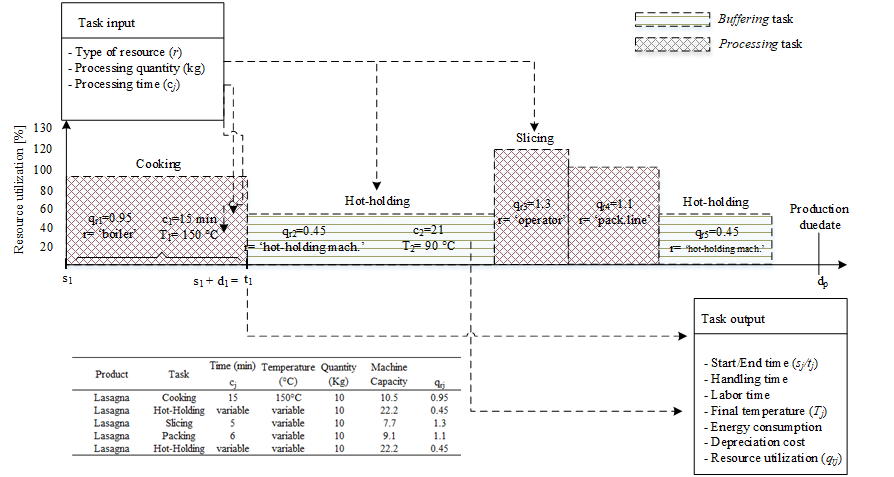
\includegraphics[width=0.9\textwidth]{sectionProduction/control_figures/fig_prod_CAMST_scheduling.png}
\captionsetup{type=figure}
\caption{Scheduling variables in a food catering plant.}
\label{fig_prod_CAMST_scheduling}
\end{figure}

In a food context, the quality is an additional constraint of the job scheduling problem; for this reason, finding the optimal solution of the model presented in \ref{secJobScheduling} becomes even more difficult since the problem is overconstrained. In addition, the minimisation of the makespan is only one of the objective function since the maximisation of the food is considered an objective as well. A multiobjective problem is proposed To meet both these purposes. It is solved by a metaheuristic algorithm called simulated annealing \cite{Reinhardt2013}.  The solutions to the problem produce the Pareto frontiers built on five daily instances (one per each production day of the input dataset). The frontiers in Figure \ref{fig_prod_CAMST_paretoFrontier} show how preserving the quality of the food product is a much more sensitive objective than the minimisation of the makespan.

% INSERT fig_prod_CAMST_paretoFrontier
\begin{figure}[hbt!]
\centering
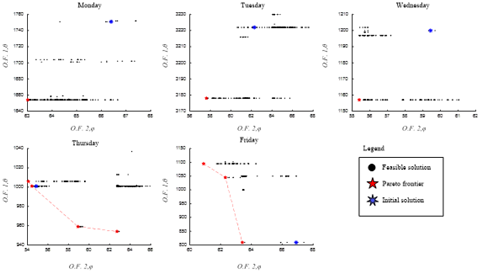
\includegraphics[width=0.9\textwidth]{sectionProduction/control_figures/fig_prod_CAMST_paretoFrontier.png}
\captionsetup{type=figure}
\caption{Pareto frontier of the bi-objective problem.}
\label{fig_prod_CAMST_paretoFrontier}
\end{figure}

Finding the best food safety solution only slightly affect the scheduling from a makespan perspective while adding significant value to the quality of the finished product. For this reason, with particular reference to the end-of-line of cook-warm product, it is crucial to design areas with hot-holder able to maintain the quality and the food safety of the products. The hot holding areas can be over-sized since their investment cost is limited but it reduces the risk of food safety and food loss due to quality and temperature decay.

\subsection{Control of a 3PL packaging plant for automotive spare parts} \label{secControlPackagingPlant}
\subsubsection{Performance assessment}

The management of this production node relies on a third-party company that perform the operations. Business processes are then fractioned, unclear, inefficient and even unknown to the managers. For this reason, the business process mapping and notation (BPMN)  is used to investigate the physical and information flows between entities and actors involved in production and planning. Figure \ref{fig_prod_CHIMAR_bpmn} illustrate an example of the BPMN together with the georeferencing of the processes on the plant layout. This technique enables visual analysis of the routes e of different processes and identifies which resources and which areas are responsible for processing a specific task. 

% INSERT fig_prod_CHIMAR_bpmn
\begin{figure}[hbt!]
\centering
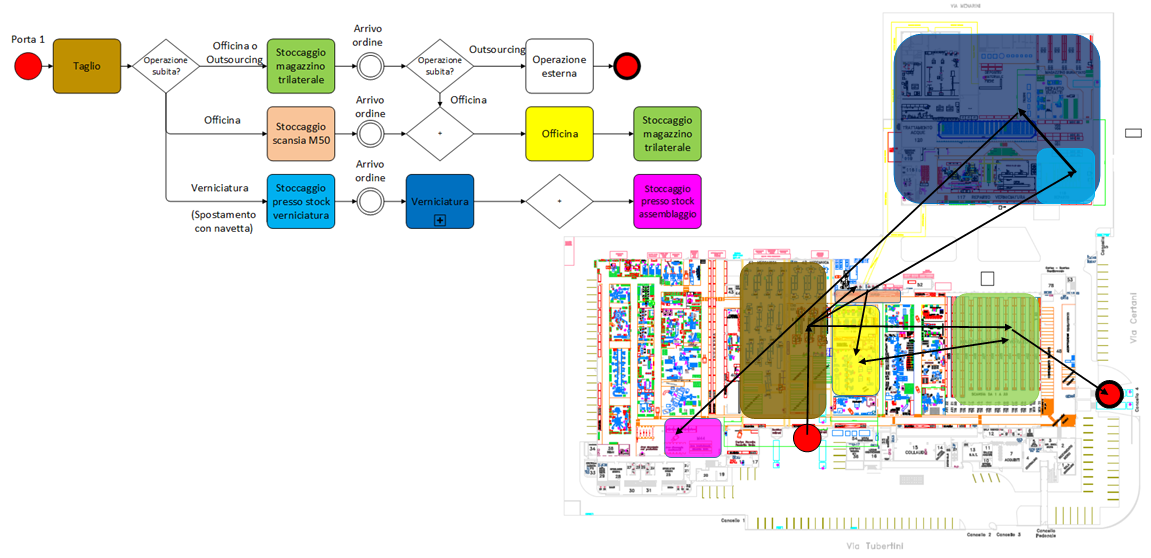
\includegraphics[width=0.9\textwidth]{sectionProduction/control_figures/fig_prod_CHIMAR_bpmn.png}
\captionsetup{type=figure}
\caption{BPMN and georeferencing of the processes operated in the 3PL packaging plant.}
\label{fig_prod_CHIMAR_bpmn}
\end{figure}

A dashboard of KPIs was defined to identify the workload and assess its impact on the working time and the distance travelled within the production site. The dashboard of KPIs in Figure \ref{fig_prod_CHIMAR_performance} shows these metrics.

% INSERT fig_prod_CHIMAR_performance
\begin{figure}[hbt!]
\centering
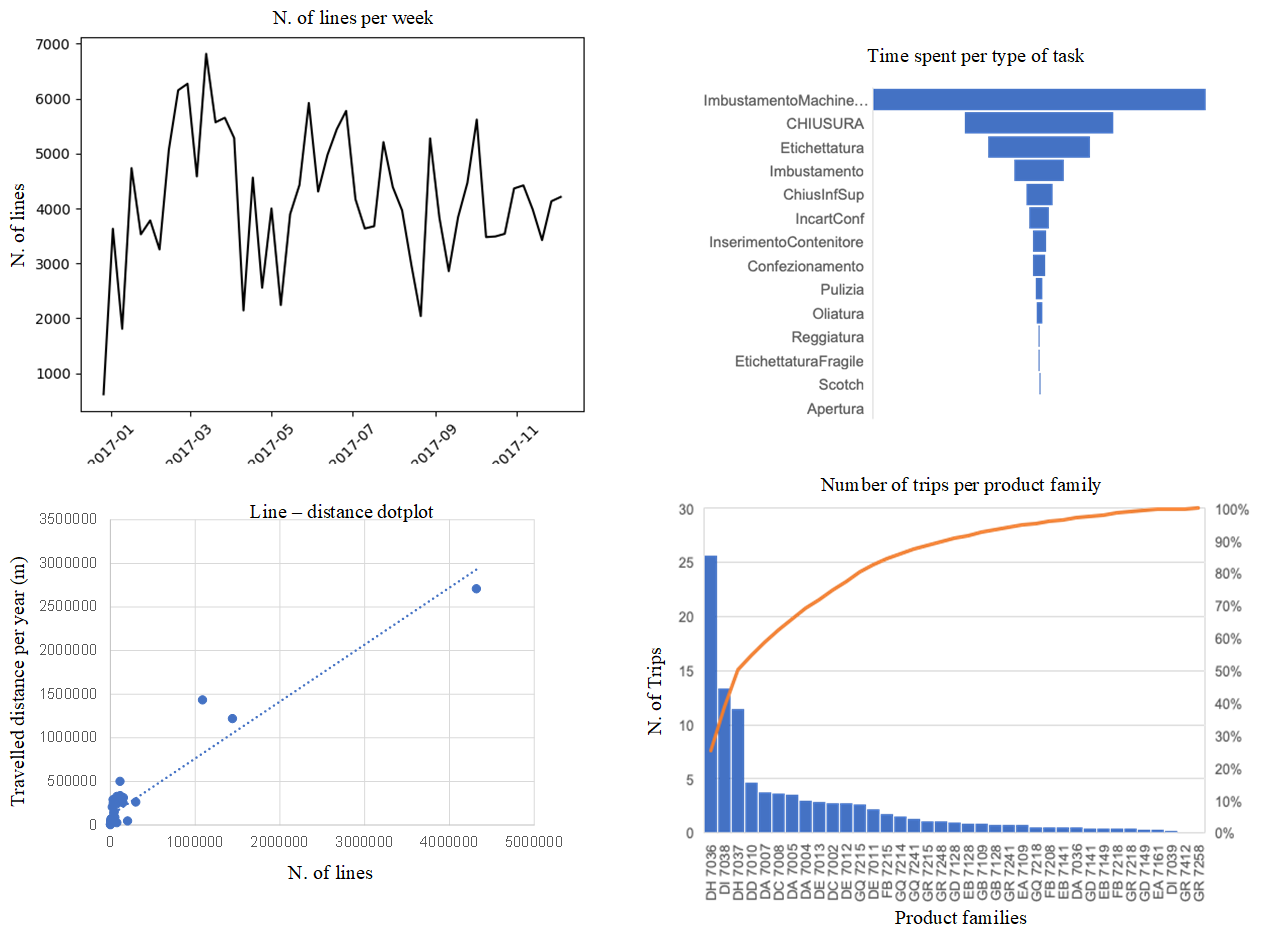
\includegraphics[width=0.7\textwidth]{sectionProduction/control_figures/fig_prod_CHIMAR_performance.png}
\captionsetup{type=figure}
\caption{Control dashboard of the processes operated in the 3PL packaging plant.}
\label{fig_prod_CHIMAR_performance}
\end{figure}

The graph in the left upper corner identifies the workload per week (number of processed lines); the bar chart in the right upper corner identifies which type of tasks are responsible for the workload in terms of time. The dot-plot in the left bottom corner identifies the trend between the number of processed lines and the distance travelled between the workstations to handle those parts. The last Pareto chart in the right bottom corner shows that a minor amount of product families is responsible for the majority of the handling activities, in terms of the distance travelled between workstations.

\subsubsection{Workload prediction}

The model in \ref{secDemandPatterns} is applied to identify demand patterns and choose the most appropriate methods to control and design the production node. Figure \ref{fig_prod_CHIMAR_demandPatterns} classifies the demand of the production system, highlighting a significant number of intermittent and lumpy parts.\footnote{The source code of Figure \ref{fig_prod_CHIMAR_demandPatterns} is available \href{https://github.com/aletuf93/logproj/blob/master/examples/PROD_02\%20Demand\%20patterns.ipynb}{here}.}

% INSERT fig_prod_CHIMAR_demandPatterns
\begin{figure}[hbt!]
\centering
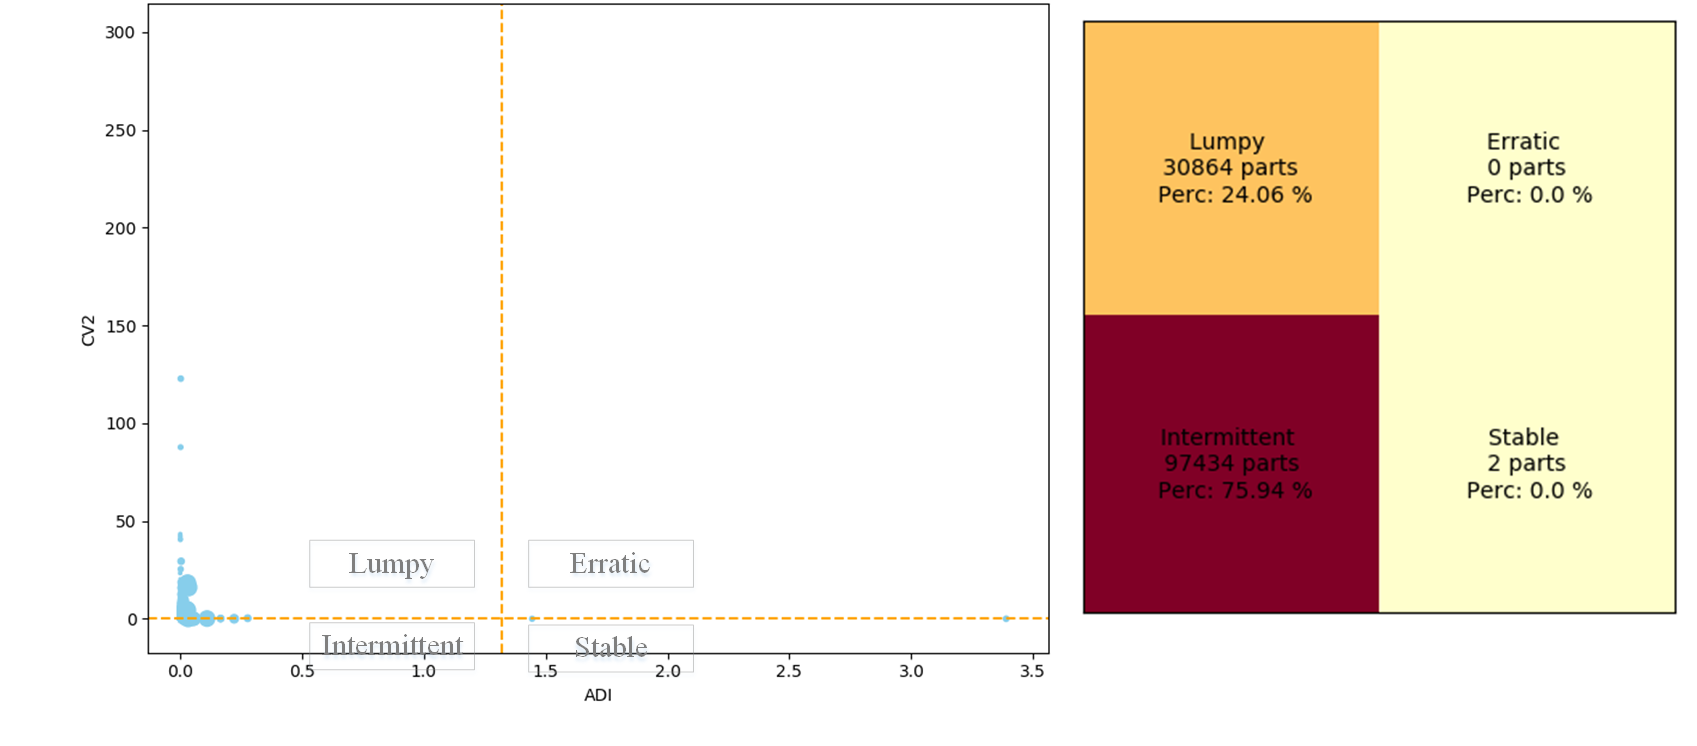
\includegraphics[width=0.7\textwidth]{sectionProduction/control_figures/fig_prod_CHIMAR_demandPatterns.png}
\captionsetup{type=figure}
\caption{Classification and patterns of the demand for a 3PL packaging plant.}
\label{fig_prod_CHIMAR_demandPatterns}
\end{figure}

Given this pattern of demand, the production node must be flexible to meet productivity variance and time requirements. In addition, demand forecast must be carefully addressed since lumpy parts have significant variance. \par

The demand trend is assessed by using descriptive analytics techniques. Figure \ref{fig_prod_CHIMAR_trend} identifies the global trends of quantities and the number of lines processed by the entire production plant. The trends are aggregated weekly and daily.\footnote{The source code of Figure \ref{fig_prod_CHIMAR_trend} is available \href{https://github.com/aletuf93/logproj/blob/master/examples/LOG_01\%20Demand\%20assessment.ipynb}{here}.}

% INSERT fig_prod_CHIMAR_trend
\begin{figure}[hbt!]
\centering
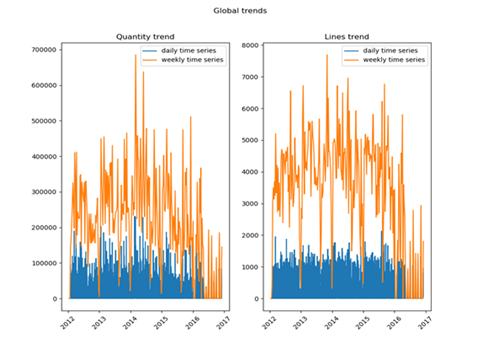
\includegraphics[width=0.7\textwidth]{sectionProduction/control_figures/fig_prod_CHIMAR_trend.png}
\captionsetup{type=figure}
\caption{Daily and weekly trend of the demand in a 3PL packaging plant.}
\label{fig_prod_CHIMAR_trend}
\end{figure}

Decomposition is applied, and the trend, seasonal and residual components are identified. Due to the length of the time series (more than six years), the series is weekly aggregated before the decomposition. 

% INSERT fig_prod_CHIMAR_decompose
\begin{figure}[hbt!]
\centering
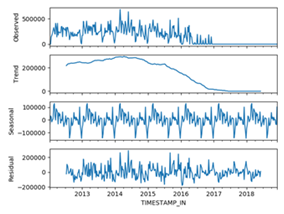
\includegraphics[width=0.7\textwidth]{sectionProduction/control_figures/fig_prod_CHIMAR_decompose.png}
\captionsetup{type=figure}
\caption{Decomposition of the market demand in a 3PL packaging plant.}
\label{fig_prod_CHIMAR_decompose}
\end{figure}

Figure \ref{fig_prod_CHIMAR_decompose} illustrates the decomposition showing a descending trend component and a seasonality occurring twice a year. The residual component is significant; this is due to the large variability of the demand already identified with the demand patterns in Figure \ref{fig_prod_CHIMAR_demandPatterns}.\footnote{The source code of Figure \ref{fig_prod_CHIMAR_decompose} is available \href{https://github.com/aletuf93/logproj/blob/master/examples/LOG_01\%20Demand\%20assessment.ipynb}{here}.} The yearly trend is predicted using the \textit{fbProphet} prediction model. Figure \ref{fig_prod_CHIMAR_fbprophet} illustrates the predictions and confidence intervals. ARIMA models cannot be applied to this time series since no transformation (square root, power, log, boxcox) leads to a stationary series. \footnote{The source code of Figure \ref{fig_prod_CHIMAR_fbprophet} is available \href{https://github.com/aletuf93/logproj/blob/master/examples/LOG_01\%20Demand\%20assessment.ipynb}{here}.}

% INSERT fig_prod_CHIMAR_fbprophet
\begin{figure}[hbt!]
\centering
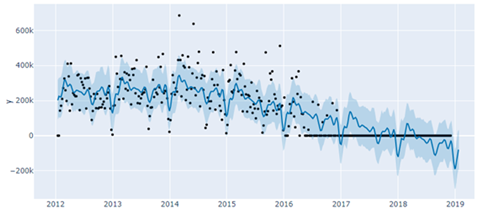
\includegraphics[width=0.7\textwidth]{sectionProduction/control_figures/fig_prod_CHIMAR_fbprophet.png}
\captionsetup{type=figure}
\caption{Prediction of the market demand in a 3PL packaging plant using the fbpropet algorithm.}
\label{fig_prod_CHIMAR_fbprophet}
\end{figure}





%\clearpage
\bibliographystyle{ieeetr}
\bibliography{sectionProduction/control_ref}



